\section{Experiments}
\label{section:experiments}

We implemented
Algorithm~\ref{algorithm:algorithm-for-strongly-linearly-separable-examples},
Algorithm~\ref{algorithm:kernelized} with
kernel~\eqref{equation:rational-kernel}, and the \textsc{Banditron} algorithm.
We generated strongly and weakly separable data sets with $K=3$ classes. The
data sets are shown in~\autoref{figure:strongly-and-weakly-separable-datasets}.
Although, the data sets are shown as two-dimensional, we used a third dimension,
the so-called \emph{constant feature}, i.e. a feature that for every example is
set to $1$. We added the constant feature so that
\autoref{figure:strongly-separable-dataset} is actually strongly lineraly
separable. For both data sets, the sample size is $T=5\times 10^6$ and the
margin is $\gamma=0.05$.

\begin{figure}[h]
\centering
\begin{subfigure}[b]{0.23\textwidth}
\captionsetup{justification=centering}
\begin{center}
\hspace*{-0.3cm} 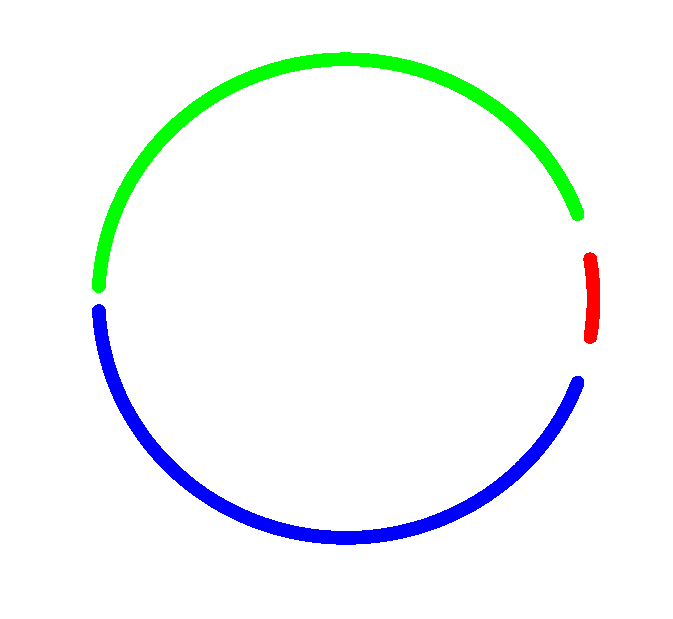
\includegraphics[width=1.15\textwidth, trim={0, 0cm, 0, 0}, clip]{figures/strong_points}
\caption{Strongly separable case}
\label{figure:strongly-separable-dataset}
\end{center}
\end{subfigure}
\hfill
\begin{subfigure}[b]{0.23\textwidth}
\captionsetup{justification=centering}
\centering
\hspace*{-0.3cm}  \includegraphics[width=1.15\textwidth, trim={0, 0cm, 0, 0}, clip]{figures/weak_points}
\caption{Weakly separable case}
\label{figure:weakly-separable-dataset}
\end{subfigure}
\vspace*{-0.2cm}
\caption{Strongly and weakly generated data sets with $K=3$ classes. All
examples lie in the unit ball of $\R^2$. Class 1 is depicted red. Classes 2 and
3 are depcited gree and blue, respectively. $80\%$ of the examples belong to class 1,
$10\%$ belong to class 2 and $10\%$ belong to class 3. Class 1
occupies the angle interval $[-15^\circ, 15^\circ]$, while classes 2 and 3
occupy angle intervals $[15^\circ, 180^\circ]$ and $[-180^\circ, -15^\circ]$
respectively. We removed points that lie within margin $\gamma=0.05$ of the
linear separator.}
\label{figure:strongly-and-weakly-separable-datasets}
\end{figure}

We evaluated all three algorithms on the two data sets. Since all three
algorithms are randomized, we run each algorithm $20$ times. \textsc{Banditron}
has exploration rate parameter $\epsilon$ for which we tried values $\epsilon
\in \{0.02, 0.01, 0.005, 0.002, 0.001, 0.0005 \}$. The average cumulative number
of mistakes up to round $t$ as a function $t$ are shown in
Figures~\ref{figure:number-of-mistakes-strongly-separable-dataset}
and~\ref{figure:number-of-mistakes-weakly-separable-dataset}.

We can see there is a dilemma for \textsc{Banditron}. When the
exploration rate $\epsilon$ is large, it suffers from the cost of exploration.
When the exploration rate is small, it cannot adapt its model quickly enough.
This problem is exacerbated when a majority class occupies a small region, like
class 1. Striking a balance between the two extremes leads to the
$\Theta(\sqrt{T})$ number of mistakes. In contrast, our algorithm makes
significant progress on every mistake it makes, leading to a finite mistake
bound.

Appendix~\ref{section:supp-to-experiment} shows decision boundaries
that each of the algorithms learns.

\begin{figure}
\centering
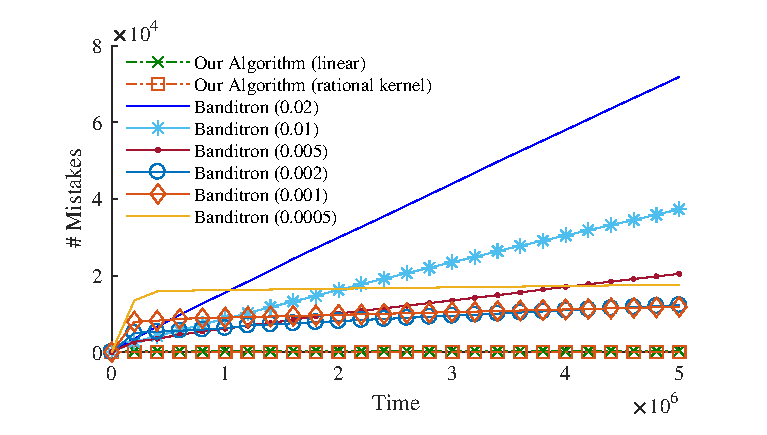
\includegraphics[width=0.45\textwidth]{figures/strong3}
\caption{Strongly separable case. Cumulative number of mistakes of various algorithms.}
\label{figure:number-of-mistakes-strongly-separable-dataset}
\end{figure}

\begin{figure}
\centering
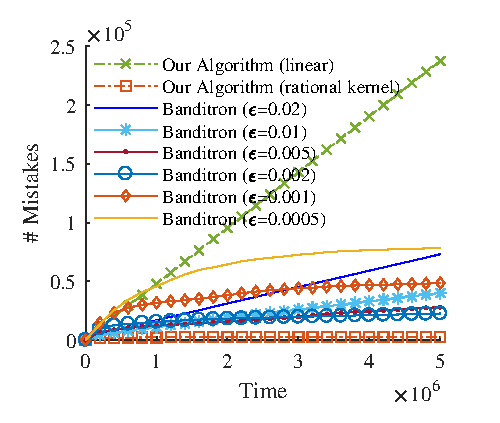
\includegraphics[width=0.45\textwidth]{figures/weak3}
\caption{Weakly separable case. Cumulative number of mistakes of various algorithms.}
\label{figure:number-of-mistakes-weakly-separable-dataset}
\end{figure}
